\documentclass[runningheads]{llncs}
\usepackage[T1]{fontenc}\usepackage{newtxtext}\usepackage[varvw]{newtxmath}
\usepackage{graphicx,amsmath,booktabs,multirow,nicefrac}\usepackage[table]{xcolor}
\usepackage[hidelinks]{hyperref}
\renewcommand{\thetable}{S\arabic{table}}\renewcommand{\thefigure}{S\arabic{figure}}
\newcommand{\Tcons}{T_{\rm cons}}
\begin{document}
\title{SelectNorm: Technical Dossier (not submitted)}
\author{[AUTHOR NAME(S)]}\institute{[AFFILIATION]}
\maketitle
\noindent Working and verification dossier for ``SelectNorm: A Disagreement-Factorized Analysis of Per-Input Normalization for Arabizi with Frozen Encoders'' (ACIIDS 2027). Values are copied unchanged from the archived tables; table and figure numbers in the main paper refer to that paper.

\begin{table}[!htb]\centering\scriptsize\setlength{\tabcolsep}{3pt}
\caption{Paired differences in macro-F1 (SelectNorm-adapt minus baseline, $\lambda=0$, seed-averaged) with 95\% paired-bootstrap intervals (10{,}000 resamples of test sentences). $^{*}$: Holm-corrected $p<0.05$ over the protocol's 20 comparisons per encoder. $^{\dagger}$: the interval lies inside $(-1,+1)$, the protocol's relevance margin; reading this as equivalence is post hoc and not corrected for multiplicity. Intervals without either mark are inconclusive about both difference and equivalence.}
\resizebox{\textwidth}{!}{\begin{tabular}{@{}llrrrr@{}}\toprule
Enc. & Set & vs.\ B1 & vs.\ B3 & vs.\ B4 & vs.\ SN-src\\\midrule
mE5 & $S_3$ & -0.71 \scriptsize[-1.25, -0.21] & -0.67 \scriptsize[-1.21, -0.17] & -0.07 \scriptsize[-0.27, +0.13]$^{\dagger}$ & -0.03 \scriptsize[-0.11, +0.06]$^{\dagger}$\\
 & $S_4$ & -0.31 \scriptsize[-0.80, +0.17]$^{\dagger}$ & -0.23 \scriptsize[-0.72, +0.25]$^{\dagger}$ & -0.03 \scriptsize[-0.25, +0.18]$^{\dagger}$ & -0.04 \scriptsize[-0.16, +0.08]$^{\dagger}$\\
 & $S_5$ & +0.39 \scriptsize[-0.22, +1.01] & +0.39 \scriptsize[-0.22, +1.01] & -0.14 \scriptsize[-0.57, +0.28]$^{\dagger}$ & -0.17 \scriptsize[-0.47, +0.11]$^{\dagger}$\\
 & $S_6$ & +0.76 \scriptsize[+0.23, +1.30] & +0.75 \scriptsize[+0.23, +1.29] & +0.02 \scriptsize[-0.22, +0.27]$^{\dagger}$ & -0.04 \scriptsize[-0.18, +0.11]$^{\dagger}$\\
\midrule
XLM-R & $S_3$ & +0.99 \scriptsize[+0.01, +2.02] & +0.91 \scriptsize[-0.07, +1.91] & +0.28 \scriptsize[+0.04, +0.52]$^{\dagger}$ & +0.07 \scriptsize[-0.02, +0.17]$^{\dagger}$\\
 & $S_4$ & -0.66 \scriptsize[-1.20, -0.11] & -0.60 \scriptsize[-1.14, -0.04] & -0.04 \scriptsize[-0.18, +0.10]$^{\dagger}$ & +0.02 \scriptsize[-0.04, +0.09]$^{\dagger}$\\
 & $S_5$ & -0.01 \scriptsize[-0.42, +0.45]$^{\dagger}$ & +0.09 \scriptsize[-0.34, +0.56]$^{\dagger}$ & -0.18 \scriptsize[-0.41, +0.03]$^{\dagger}$ & -0.25 \scriptsize[-0.45, -0.07]$^{*}$$^{\dagger}$\\
 & $S_6$ & -3.76 \scriptsize[-4.58, -2.93]$^{*}$ & -3.77 \scriptsize[-4.58, -2.94]$^{*}$ & -0.23 \scriptsize[-0.42, -0.03]$^{\dagger}$ & +0.53 \scriptsize[+0.33, +0.73]$^{*}$$^{\dagger}$\\
\midrule
LaBSE & $S_3$ & -0.19 \scriptsize[-0.75, +0.35]$^{\dagger}$ & -0.24 \scriptsize[-0.73, +0.23]$^{\dagger}$ & +0.03 \scriptsize[-0.19, +0.24]$^{\dagger}$ & +0.03 \scriptsize[-0.08, +0.14]$^{\dagger}$\\
 & $S_4$ & -0.37 \scriptsize[-1.01, +0.28] & -0.35 \scriptsize[-0.95, +0.25]$^{\dagger}$ & +0.15 \scriptsize[-0.06, +0.34]$^{\dagger}$ & +0.01 \scriptsize[-0.11, +0.14]$^{\dagger}$\\
 & $S_5$ & +0.62 \scriptsize[-1.20, +2.44] & +0.57 \scriptsize[-1.17, +2.32] & -0.07 \scriptsize[-0.60, +0.47]$^{\dagger}$ & +0.34 \scriptsize[-0.01, +0.71]$^{\dagger}$\\
 & $S_6$ & +5.46 \scriptsize[+4.44, +6.50]$^{*}$ & +5.04 \scriptsize[+4.05, +6.04]$^{*}$ & +0.32 \scriptsize[+0.06, +0.58]$^{\dagger}$ & +0.54 \scriptsize[+0.30, +0.79]$^{*}$$^{\dagger}$\\
\midrule
MARBERTv2 & $S_3$ & -0.01 \scriptsize[-0.65, +0.64]$^{\dagger}$ & -0.16 \scriptsize[-0.77, +0.48]$^{\dagger}$ & +0.03 \scriptsize[-0.18, +0.23]$^{\dagger}$ & -0.09 \scriptsize[-0.20, +0.01]$^{\dagger}$\\
 & $S_4$ & +0.57 \scriptsize[+0.08, +1.06] & +0.16 \scriptsize[-0.37, +0.68]$^{\dagger}$ & +0.06 \scriptsize[-0.10, +0.22]$^{\dagger}$ & +0.00 \scriptsize[-0.07, +0.08]$^{\dagger}$\\
 & $S_5$ & +0.58 \scriptsize[-0.45, +1.64] & +0.58 \scriptsize[-0.45, +1.64] & -0.11 \scriptsize[-0.63, +0.40]$^{\dagger}$ & -0.01 \scriptsize[-0.36, +0.35]$^{\dagger}$\\
 & $S_6$ & -0.53 \scriptsize[-1.15, +0.08] & -0.61 \scriptsize[-1.22, -0.01] & +0.12 \scriptsize[-0.19, +0.43]$^{\dagger}$ & -0.01 \scriptsize[-0.15, +0.12]$^{\dagger}$\\
\bottomrule\end{tabular}
}\end{table}

\begin{table}[!htb]\centering\scriptsize\setlength{\tabcolsep}{3.5pt}
\caption{As Table~2 of the paper, with $f$ also trained on synthetic Latin renderings (\textsc{+syn}, exploratory regime).}
\resizebox{\textwidth}{!}{\begin{tabular}{@{}lrrrrrrrr@{}}\toprule
 & \multicolumn{4}{c}{\textbf{mE5+syn}} & \multicolumn{4}{c}{\textbf{XLM-R+syn}}\\
\cmidrule(lr){2-5}\cmidrule(lr){6-9}
 & $S_3$ & $S_4$ & $S_5$ & $S_6$ & $S_3$ & $S_4$ & $S_5$ & $S_6$\\\midrule
B0 original & 80.9$^{\triangledown}$ & 65.6$^{\triangledown}$ & 69.1 & \textbf{61.5} & 69.0$^{\triangledown}$ & 59.8$^{\triangledown}$ & 64.7 & 59.7\\
B1 always normalise & 81.6 & 67.5 & 72.6 & 58.0$^{\triangledown}$ & 72.8 & 63.2 & 62.9 & 59.1\\
B2 random, matched rate & 81.2 & 66.5 & 70.4 & 61.0 & 70.8 & 61.6 & 63.9 & 59.7\\
B3 confidence threshold & 83.0 & 68.7 & \textbf{73.2} & 60.7 & 74.5 & 63.0 & 64.7 & 60.3\\
B4 direct gain & \textbf{83.8} & \textbf{68.9} & 72.4 & 60.9 & \textbf{74.5} & 63.8 & 65.1 & 60.6\\
B4b per-view loss & 83.8 & 68.9 & 72.5 & 60.8 & 74.3 & 63.8 & 65.0 & 60.5\\
SelectNorm-src & 83.6 & 68.8 & 72.9 & 61.1 & 74.3 & 63.5 & \textbf{65.5} & 60.4$^{\triangledown}$\\
\rowcolor{black!6}SelectNorm-adapt & 83.7 & 68.9 & 73.0 & 61.1 & 74.3 & 63.5 & 65.4 & 60.6\\
\quad Bayes threshold $\lambda\bar c$ & 83.7 & 68.8 & 73.2 & 61.1 & 74.5 & \textbf{63.9} & 65.0 & \textbf{60.8}\\
\addlinespace[2pt]
R two-view ensemble$^\dagger$ & 83.7 & 68.9 & 74.7 & 60.5 & 75.8 & 64.0 & 65.6 & 60.7\\
B6 oracle$^\ddagger$ & 91.7 & 80.9 & 85.7 & 71.4 & 86.3 & 79.0 & 80.6 & 73.5\\
\midrule[\heavyrulewidth]
 & \multicolumn{4}{c}{\textbf{LaBSE+syn}} & \multicolumn{4}{c}{\textbf{MARBERTv2+syn}}\\
\cmidrule(lr){2-5}\cmidrule(lr){6-9}
 & $S_3$ & $S_4$ & $S_5$ & $S_6$ & $S_3$ & $S_4$ & $S_5$ & $S_6$\\\midrule
B0 original & 76.6$^{\triangledown}$ & 64.9$^{\triangledown}$ & 71.3 & \textbf{62.4}$^{\blacktriangle}$ & 77.0$^{\triangledown}$ & 64.2$^{\triangledown}$ & 57.0 & 50.1$^{\triangledown}$\\
B1 always normalise & 83.7 & 67.8 & 74.3 & 58.7$^{\triangledown}$ & 81.8 & 67.8$^{\triangledown}$ & 59.3 & \textbf{60.7}$^{\blacktriangle}$\\
B2 random, matched rate & 80.3 & 66.3 & 72.9 & 59.9 & 80.8 & 67.3 & 59.1 & 58.3\\
B3 confidence threshold & \textbf{84.3} & 68.2 & 74.3 & 60.4 & 82.9 & 68.7 & 59.3 & 59.5$^{\blacktriangle}$\\
B4 direct gain & 84.3 & \textbf{68.5} & 74.4 & 59.7 & 82.5 & 68.7 & 59.6 & 59.3$^{\blacktriangle}$\\
B4b per-view loss & 84.1 & 68.5 & \textbf{74.8} & 59.6 & 82.3 & 68.7 & 59.6 & 58.7\\
SelectNorm-src & 84.1 & 68.3 & 74.7 & 60.0 & 82.5 & 68.8 & 59.8 & 59.0\\
\rowcolor{black!6}SelectNorm-adapt & 84.2 & 68.2 & 74.6 & 60.0 & 82.6 & 68.9 & \textbf{59.9} & 58.9\\
\quad Bayes threshold $\lambda\bar c$ & 84.2 & 68.2 & 74.8 & 60.1 & \textbf{83.0} & \textbf{69.2} & 59.8 & 58.6\\
\addlinespace[2pt]
R two-view ensemble$^\dagger$ & 83.5 & 68.8 & 76.6 & 61.3 & 83.6 & 69.0 & 59.3 & 57.3\\
B6 oracle$^\ddagger$ & 92.9 & 81.1 & 86.8 & 73.1 & 92.6 & 81.6 & 72.3 & 69.3\\
\bottomrule\end{tabular}
}\end{table}

\begin{table}[!htb]\centering\footnotesize\setlength{\tabcolsep}{3pt}
\caption{Routing behaviour (mE5, $\lambda=0$): selection rate, harmful transformations per 100 inputs, share of oracle opportunities captured, and estimated cost relative to B0. Help/harm: number of inputs where normalisation corrects/introduces an error.}
\resizebox{\textwidth}{!}{\begin{tabular}{@{}lrrrrrrrrrrrrrrrr@{}}\toprule
 & \multicolumn{4}{c}{$S_3$ \scriptsize(help 376, harm 114)} & \multicolumn{4}{c}{$S_4$ \scriptsize(help 538, harm 402)} & \multicolumn{4}{c}{$S_5$ \scriptsize(help 124, harm 89)} & \multicolumn{4}{c}{$S_6$ \scriptsize(help 407, harm 456)}\\\cmidrule(lr){2-5}\cmidrule(lr){6-9}\cmidrule(lr){10-13}\cmidrule(lr){14-17}
System & Sel.\,\% & Harm & Capt.\,\% & Cost & Sel.\,\% & Harm & Capt.\,\% & Cost & Sel.\,\% & Harm & Capt.\,\% & Cost & Sel.\,\% & Harm & Capt.\,\% & Cost\\\midrule
B1 & 100.0 & 8.0 & 100.0 & 0.98 & 100.0 & 14.0 & 100.0 & 0.97 & 100.0 & 12.2 & 100.0 & 0.98 & 100.0 & 10.9 & 100.0 & 1.04\\
B3 & 98.9 & 8.0 & 99.7 & 1.97 & 99.1 & 14.0 & 99.5 & 1.97 & 99.5 & 12.2 & 100.0 & 1.97 & 98.5 & 10.9 & 99.9 & 2.03\\
B4 & 90.2 & 7.6 & 96.1 & 1.89 & 88.8 & 13.1 & 93.8 & 1.87 & 86.4 & 10.9 & 95.5 & 1.84 & 66.8 & 7.9 & 76.9 & 1.70\\
SN-adapt & 89.0 & 7.6 & 95.7 & 1.88 & 87.0 & 13.0 & 93.3 & 1.86 & 85.7 & 11.3 & 96.8 & 1.83 & 65.9 & 8.3 & 80.9 & 1.69\\
Oracle & 26.4 & 0.0 & 100.0 & 1.26 & 18.7 & 0.0 & 100.0 & 1.18 & 17.0 & 0.0 & 100.0 & 1.17 & 9.7 & 0.0 & 100.0 & 1.10\\
\bottomrule\end{tabular}
}\end{table}

\begin{table}[!htb]\centering\scriptsize\setlength{\tabcolsep}{4pt}
\caption{95\% intervals for the mechanism measurements of Table~3 of the paper (1{,}000 bootstrap resamples of test sentences, seed-averaged within each resample; estimators not refitted).}
\resizebox{\textwidth}{!}{\begin{tabular}{@{}llllllll@{}}\toprule
Enc. & Set & AUC$_\pi$ & AUC$_\rho$ & AUC$_\rho^{\rm tgt}$ & gap (pts) & $\Delta_{\rm src}$ & $\Delta_{\rm tgt}$\\\midrule
mE5 & $S_3$ & [0.65, 0.71] & [0.60, 0.72] & [0.58, 0.69] & [-0.8, +6.8] & [-1.0, -0.2] & [-0.8, +0.7]\\
 & $S_4$ & [0.62, 0.66] & [0.52, 0.60] & [0.54, 0.61] & [+15.2, +21.9] & [-0.8, +0.1] & [-1.2, +1.0]\\
 & $S_5$ & [0.57, 0.66] & [0.55, 0.71] & [0.49, 0.64] & [+7.7, +21.1] & [-0.2, +0.5] & [-1.5, +2.9]\\
 & $S_6$ & [0.73, 0.76] & [0.50, 0.57] & [0.52, 0.60] & [+16.7, +23.5] & [-1.7, +0.6] & [-0.7, +0.9]\\
\midrule
XLM-R & $S_3$ & [0.61, 0.67] & [0.66, 0.76] & [0.63, 0.73] & [-0.8, +6.2] & [+0.1, +2.0] & [-0.3, +2.0]\\
 & $S_4$ & [0.64, 0.68] & [0.53, 0.60] & [0.53, 0.61] & [+8.0, +14.6] & [-0.9, +0.0] & [-0.2, +0.8]\\
 & $S_5$ & [0.65, 0.74] & [0.35, 0.53] & [0.50, 0.69] & [+4.5, +18.0] & [+0.0, +0.7] & [-2.1, +0.8]\\
 & $S_6$ & [0.71, 0.74] & [0.41, 0.48] & [0.63, 0.70] & [-10.9, -4.7] & [-4.0, -2.5] & [+0.6, +1.7]\\
\midrule
LaBSE & $S_3$ & [0.66, 0.72] & [0.55, 0.67] & [0.47, 0.60] & [-4.5, +3.7] & [-0.4, +0.6] & [-0.6, +0.3]\\
 & $S_4$ & [0.63, 0.67] & [0.54, 0.61] & [0.55, 0.62] & [+3.0, +8.9] & [-1.0, +0.2] & [-1.2, +0.3]\\
 & $S_5$ & [0.61, 0.69] & [0.52, 0.66] & [0.48, 0.62] & [-2.9, +9.6] & [-1.3, +2.1] & [-2.0, +2.4]\\
 & $S_6$ & [0.67, 0.70] & [0.54, 0.60] & [0.61, 0.68] & [+13.0, +18.5] & [-3.8, -1.3] & [+0.2, +1.3]\\
\midrule
MARBERTv2 & $S_3$ & [0.66, 0.72] & [0.59, 0.69] & [0.55, 0.66] & [-2.2, +5.3] & [-0.4, +0.6] & [-1.2, +0.5]\\
 & $S_4$ & [0.69, 0.73] & [0.58, 0.65] & [0.61, 0.68] & [+10.0, +15.7] & [-0.1, +0.9] & [+1.6, +3.9]\\
 & $S_5$ & [0.70, 0.77] & [0.55, 0.69] & [0.47, 0.62] & [+7.0, +19.8] & [-1.9, +1.2] & [-1.3, +2.9]\\
 & $S_6$ & [0.69, 0.72] & [0.52, 0.58] & [0.59, 0.66] & [+1.7, +7.1] & [-0.9, +0.3] & [+0.3, +1.8]\\
\bottomrule\end{tabular}
}\end{table}

\begin{table}[!htb]\centering\scriptsize\setlength{\tabcolsep}{3pt}
\caption{Sensitivity of the oracle reference (range over the four sets). ``Views headroom'': oracle over $x$ and $T(x)$ minus the best view; other columns: the same for two classifiers differing only in their training sample (bootstrap as in Table~3 of the paper, 80\%/50\% subsamples, or bootstrap with $C\times3$ or $C/3$), applied to $x$; mean of 10 pairs.}
\resizebox{\textwidth}{!}{\begin{tabular}{@{}lrrrrrr@{}}\toprule
 & views & \multicolumn{5}{c}{reference headroom (two resampled classifiers)}\\
\cmidrule(lr){3-7}
Enc. & headroom & bootstrap & 80\% sub. & 50\% sub. & boot., $3C$ & boot., $C/3$\\\midrule
mE5 & 8.0--14.1 & 6.1--9.1 & 2.9--4.0 & 4.8--6.8 & 8.0--10.9 & 4.2--7.3\\
XLM-R & 7.3--10.7 & 3.4--5.1 & 2.1--3.0 & 1.7--3.6 & 5.1--7.2 & 2.0--4.2\\
LaBSE & 7.9--14.9 & 6.6--7.4 & 3.3--3.9 & 6.1--7.0 & 7.2--8.6 & 5.4--6.2\\
MARBERTv2 & 11.5--16.5 & 10.6--15.3 & 4.7--6.3 & 9.4--14.5 & 14.8--21.9 & 8.2--11.3\\
\bottomrule\end{tabular}
}\end{table}

\begin{table}[!htb]\centering\footnotesize\setlength{\tabcolsep}{4pt}
\caption{Net effect of always normalising (help minus harm per 100 inputs) by input condition, mean over the four encoders, range in brackets. Conditions were fixed before inspection.}
\resizebox{\textwidth}{!}{\begin{tabular}{@{}lrrrr@{}}\toprule
Condition (share of $S_3$/$S_4$/$S_5$/$S_6$) & $S_3$ & $S_4$ & $S_5$ & $S_6$\\\midrule
French/English $\ge$30\% (9/12/12/22) & +4.3 \scriptsize[+0,+11] & +4.3 \scriptsize[-2,+13] & +1.6 \scriptsize[-3,+5] & -0.1 \scriptsize[-9,+7]\\
not French/English $\ge$30\% (91/88/88/78) & +17.0 \scriptsize[+15,+20] & +7.6 \scriptsize[+5,+9] & +6.5 \scriptsize[+5,+10] & +1.3 \scriptsize[-11,+12]\\
negation rule applied (8/12/26/6) & +14.0 \scriptsize[+6,+18] & +5.9 \scriptsize[-4,+20] & +4.0 \scriptsize[-4,+9] & +2.1 \scriptsize[-9,+15]\\
not negation rule applied (92/88/74/94) & +16.1 \scriptsize[+14,+18] & +7.4 \scriptsize[+6,+11] & +6.5 \scriptsize[+3,+11] & +1.0 \scriptsize[-11,+10]\\
lexicon coverage $<$50\% (51/57/81/85) & +12.3 \scriptsize[+11,+14] & +4.5 \scriptsize[+2,+9] & +3.7 \scriptsize[+1,+6] & +0.8 \scriptsize[-11,+11]\\
not lexicon coverage $<$50\% (49/43/19/15) & +19.7 \scriptsize[+17,+23] & +10.8 \scriptsize[+9,+14] & +15.1 \scriptsize[+8,+22] & +2.4 \scriptsize[-11,+13]\\
$\le$3 tokens (42/28/2/27) & +14.2 \scriptsize[+10,+16] & +8.4 \scriptsize[+0,+15] & +13.2 \scriptsize[-18,+35] & +0.7 \scriptsize[-10,+10]\\
not $\le$3 tokens (58/72/98/73) & +17.2 \scriptsize[+13,+20] & +6.8 \scriptsize[+3,+10] & +5.7 \scriptsize[+4,+10] & +1.2 \scriptsize[-11,+11]\\
\bottomrule\end{tabular}
}\end{table}

\begin{table}[!htb]\centering\footnotesize\setlength{\tabcolsep}{3pt}
\caption{Ablations (mE5, $\lambda=0$, macro-F1, mean of five seeds). Rows with ``always'' are B1 with that normaliser.}
\begin{tabular}{@{}lrrrr@{}}\toprule
Variant & $S_3$ & $S_4$ & $S_5$ & $S_6$\\\midrule
SelectNorm-adapt (full) & 81.3 & 66.9 & 69.8 & 53.7\\
\quad -- target re-estimation of $\hat\pi$ & 81.3 & 67.0 & 70.0 & 53.7\\
\quad Bayes threshold instead of tuned & 81.4 & 66.9 & 69.6 & 53.5\\
\quad $2\hat\rho-1$ only (no $\hat\pi$) & 81.3 & 66.9 & 69.8 & 53.6\\
\quad $\hat\pi$ only, tuned (label-free ranking) & 81.9 & 67.2 & 69.5 & 53.1\\
\quad confidence features only & 82.0 & 67.2 & 69.4 & 53.0\\
\quad -- confidence features & 81.5 & 66.9 & 69.6 & 53.6\\
\quad -- script features & 81.6 & 67.1 & 69.8 & 53.4\\
\quad -- normaliser reliability & 82.0 & 67.0 & 69.4 & 53.2\\
\quad + embedding PCA & 82.0 & 67.2 & 70.9 & 53.8\\
\quad gradient boosting & 82.0 & 67.1 & 69.6 & 53.1\\
\quad $T_{\rm lex}$ (no safeguards) & 80.7 & 64.6 & 65.2 & 53.0\\
\quad always $T_{\rm lex}$ & 77.8 & 61.8 & 63.2 & 47.9\\
\quad $T_{\rm rule}$ & 76.7 & 61.8 & 61.4 & 53.3\\
\quad always $T_{\rm rule}$ & 75.1 & 58.8 & 58.8 & 47.7\\
\quad $T_{\rm cov}$ (unknown tokens kept Latin) & 75.0 & 65.7 & 70.8 & 54.1\\
\quad always $T_{\rm cov}$ & 75.0 & 65.8 & 70.7 & 54.0\\
\bottomrule\end{tabular}
\end{table}

\begin{table}[!htb]\centering\footnotesize\setlength{\tabcolsep}{2.5pt}
\caption{Normaliser accuracy against human Arabic-script transliterations: \emph{development} results, not an independent test. TArC: 20\% of sentences, not used for the lexicon $\mathcal L$ but used to design the safeguards. NArabizi: whole corpus, nothing fitted to it, but scored during development. ``Foreign kept'': precision/recall of keeping annotated French/English tokens in Latin script; negation: accuracy on circumfix-negated verbs. Audit: no hand-listed word occurs only in the development split; on the 87\% of tokens no rule touches, word accuracy is 65.8\%; with the splits' roles swapped, negation is kept in 94.4\% and foreign precision/recall is 95/77.}
\resizebox{\textwidth}{!}{\begin{tabular}{@{}lrrrrr@{}}\toprule
 & \multicolumn{3}{c}{TArC development split (Tunisian)} & \multicolumn{2}{c}{NArabizi (Algerian, out of dialect)}\\\cmidrule(lr){2-4}\cmidrule(lr){5-6}
Strategy & Word acc. & Foreign kept (P/R) & Negation & Word acc. & Foreign kept (P/R)\\\midrule
$T_{\rm rule}$ & 36.3 & --/0 & 29.1 & 39.0 & --/0\\
$T_{\rm lex}$ & 69.5 & --/0 & 54.4 & 47.6 & --/0\\
$T_{\rm cons}$ & 69.1 & 96/79 & 96.1 & 46.8 & 93/53\\
\bottomrule\end{tabular}
}\end{table}

\begin{figure}[!htb]\centering
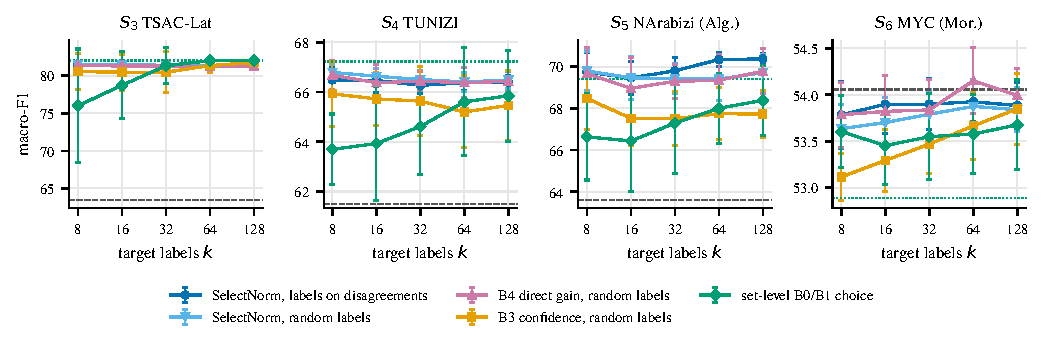
\includegraphics[width=\textwidth]{../figures/fewlabel.pdf}
\caption{Few-label adaptation (mE5): macro-F1 against the number $k$ of labelled target sentences (5 draws $\times$ 5 seeds; error bars: s.d.). Dashed: B0; dotted: B1. ``Set-level choice'' picks B0 or B1 by accuracy on the $k$ labels.}
\end{figure}
\clearpage
\section*{Implementation details}
\paragraph{Encoders and software.} Encoders are loaded at pinned revisions with SHA-256-verified weights: XLM-R base \texttt{e73636d} (MIT), mE5 base \texttt{d128750} (MIT), LaBSE \texttt{836121a} (Apache-2.0), MARBERTv2 \texttt{fe88db9} (no licence stated). Representations: mean of the last layer over non-padding tokens, at most 128 subwords, $\ell_2$-normalised; mE5 inputs carry \texttt{query:}. Python 3, scikit-learn 1.9.1, NumPy 2.5.3; code, configuration, logs and the protocol are released.

\paragraph{Classifier $f$.} $\ell_2$-regularised logistic regression; $C\in\{0.01,0.03,\ldots,100\}$ selected by macro-F1 on TSAC-\textsc{ar} dev; temperature fitted on the same split by NLL. The \textsc{+syn} regime adds the synthetic Latin rendering $G(x)$ of every training and dev sentence.

\paragraph{Router.} $\hat\pi,\hat\rho$: logistic regression on standardised $z$ ($C=1$); 17 features: confidence, margin and entropy of $p_0$ (\textsc{conf}); length, Latin and Arabic shares, digit-as-letter, emoji and upper-case rates (\textsc{script}); lexicon, rule-fallback, ambiguity, protected, negation, laughter and changed-token rates and lexicon entropy of $T$ (\textsc{trel}). Policy split 80/20 of TSAC-\textsc{lat} train with seed $1000+s$; the 20\% part tunes thresholds. 

\paragraph{Few-label audit.} \texttt{check\_fewlabel.py} replays every targeted and random label draw of all eight encoder--regime runs (8{,}000 draws), saves the sampled source identifiers, and counts any sampled label from the scored fold, any shared source identifier or normalised text between sampled and scored sentences, and any targeted sentence that is not a disagreement: none. A rerun of \texttt{adapt.py} for mE5 with index logging matches the replay in all 1{,}000 draws and the archived results in all 2{,}500 rows. In 375 targeted draws ($S_5$, $k{=}128$) fewer than $k$ disagreements were available.

\paragraph{Per-example exports.} \texttt{results/export/per\_example} gives, per encoder, regime and set, sentence and source identifiers, labels, both views' probabilities and every system's $\lambda{=}0$ prediction per seed. \texttt{scripts/reproduce\_stats.py} (NumPy and pandas only) recomputes from them every difference, interval and $p$-value of Table~2 of the paper and Table~S1 for all four encoders exactly.

\paragraph{Costs.} $c_T$ is the measured normaliser time (about 0.4\% of a pass). $c_0,c_1$ are \emph{estimated} per sentence by a per-encoder model $a+b\cdot$tokens fitted to measured batch-1 latencies of 300 sentences per set and view (e.g.\ mE5 $a=19.6$\,ms, $b=0.32$\,ms/token, $R^2=0.68$), as used in Fig.~2 of the paper and Table~S3. \texttt{measured\_cost.py} runs the deployed pipeline on raw text at batch size 1 with nothing cached (pinned encoder, the trained head refitted deterministically, which reproduces the cached probabilities exactly, normaliser, features, each seed's router and $\lambda{=}0$ threshold, second pass only when selected). On all 9{,}220 test sentences, none of the 184{,}400 live routing decisions (4 encoders $\times$ 5 seeds) or final predictions differs from the archived ones (probabilities within $1.6\cdot10^{-4}$). Timed back to back on 200 sentences per set: B0 22--31\,ms; relative costs within $-0.02$ to $+0.05$ of the estimates for B1 and R, $+0.03$ to $+0.07$ for SelectNorm (features are not in the token model). mE5 was re-timed after a concurrent job overlapped it (both runs archived).
\end{document}
